% Figure 1: authors' hierarchy-only mechanism diagram (ServeSID_figures_no_pairloss).
\begin{figure*}[t]
\centering
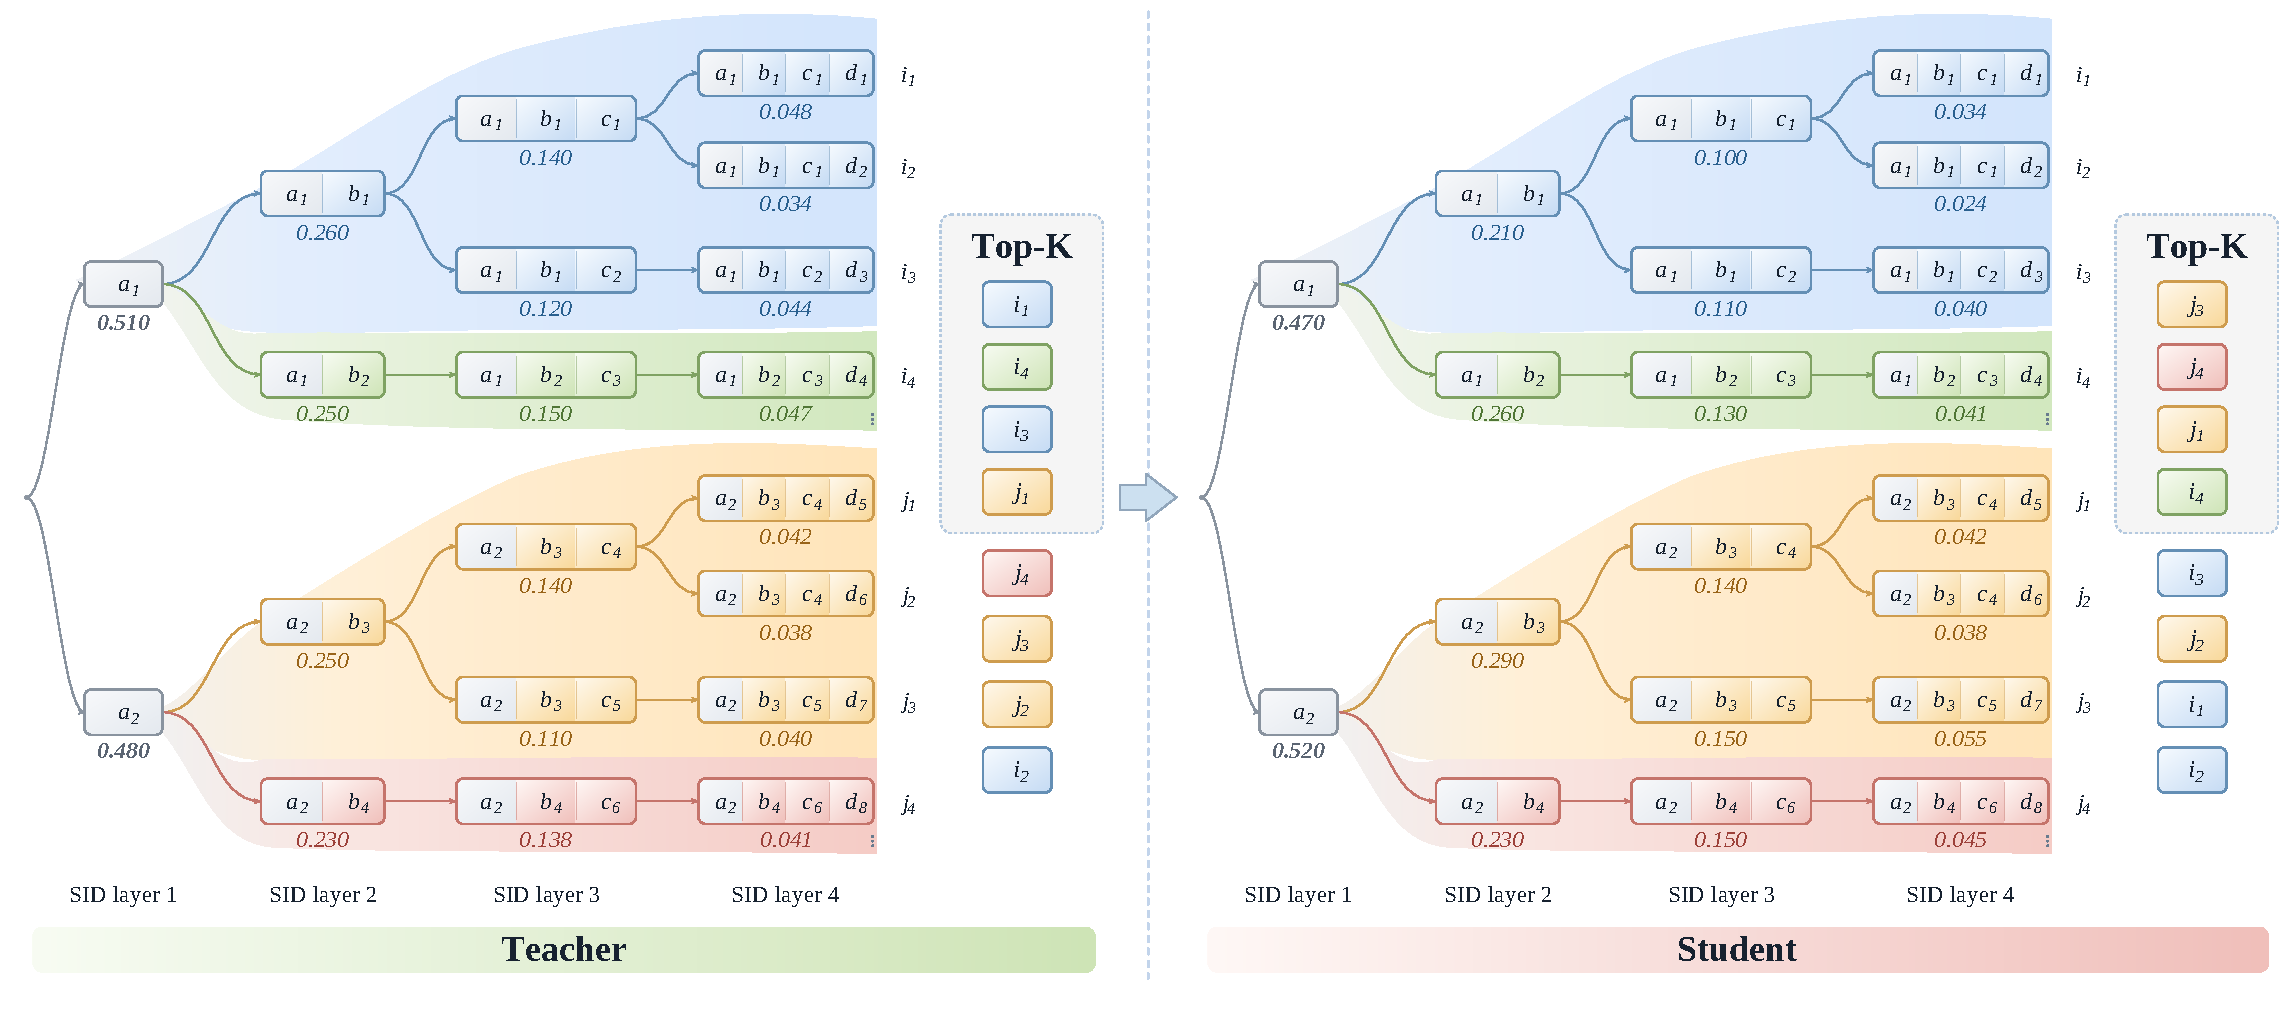
\includegraphics[width=0.945\textwidth]{Figures/diag_hierarchy.pdf}
\caption{Teacher and student complete-SID rankings on selected
identifier paths. Node labels show cumulative log-scores (sums
of conditional log-probabilities), not normalized prefix masses.
HServe normalizes the completed candidate scores on a common
support and then sums their probabilities within shared-prefix groups.}
\Description{Teacher and student SID trees show selected paths, cumulative
log-scores and candidate orders. The displayed node scores are not
normalized HServe prefix marginals.}
\label{fig:hierarchical}
\end{figure*}
